\chapter{IOSharp}\label{C:IOSharp development}

In this chapter it will be explained how was defined and architected, designed and implemented the core of IOSharp disaggregating the different parts and explaining each one.
\\
\\
First of all it will be explained the project design explaining which two options where at project definition, then the implementation is explained for the different IO ports and communication standards used in this project. Finally, it will be explained how is done the port mapping to work between different boards and devices.

\section{Planning the development}\label{S:Design}
At project start, the development was focused on a tiny Linux board called RaspberryPi. This device was designed by RaspberryPi Foundation in England taking in mind the kids around the world and helping them to provide cheap tools to be introduced in computer science. It is an interesting board for its features, offering basic IO using the provided GPIOs, it also provides a SPI module for peripheral communication, an I$^{2}$C and UART interface also for transmissions between external components and the device itself.
\\
In addition to the interfaces mentioned above, it also has some desktop interesting features like USB ports which practically can accept any device that works on Linux for instance a WiFi, Bluetooth, ZigBee or any stick for wireless transmissions, HDMI for graphics and user interface and Ethernet for network communications. Apart from this IO characteristics, it also mounts a decent ARMv6 (CPU) running at 700MHz on stock frequency and being overclocked to 1GHz without problems. Together with the CPU 512MB of RAM are provided which is enough for normal desktop usage (surfing, emailing and office) and for embedded projects.
\\
\\
After choosing the target device, two implementing options where designed and analysed. Each one has its own benefits and problems that are going to be explained in the following sections. As an introduction to the options that were considered where the use of the specific tools and libraries for the RaspberryPi and its CPU, this should help on achieving high efficiency when deployed on the device. On the other hand, trying to develop the project as widely as possible to give the chance of running under any Linux (or similar operating systems like Unix or Android) avoiding the exclusion of other devices.

\subsection{Focused on RaspberryPi}\label{SS:}
\subsection{Focused on Linux in General}\label{SS:}
Since the design of IOSharp was focused on reach any device capable of execute C\# and not only the RasperryPi the best solution could be use 

\section{Implementation}\label{S:Implementation}
Remember that as it was explained on the introduction, the goal of this thesis is deploy and run successfully the HomeSense platform on a RaspberryPi. Taking in mind this, some modules where required to develop in order to accomplish with this requirement. In this case the GPIO, Interrupts, SPI and UART need to work in order to use the different components of HomeSense.

\subsection{GPIO}\label{SS:GPIO}
In order to implement the GPIO ports in NETMF it will be used the IOPorts.cs file which contain the structure for Input, Output, Tristate and Interrupt ports, the first three will be explained in this section whereas the interrupt port will have a dedicated one.
\\
Below is explained the different options on implementing GPIOs in Linux, which has been chosen and how has been implemented in this project.

\subsubsection{Implementation Options}\label{SSS:Implementation-Options}
GPIO acronym stands for General Purpose Input Output which are Ports on systems that are capable of generating an output or reading an input. Normally embedded systems work with ports at 3.3V, other devices had low power supply like 2V. And it is not strange that many of them are tolerant to 5V in input.
\\
In case of the Netduino and RaspberryPi the ports on both devices run at 3.3V and also the different test hardware modules used in this thesis.
\\
\\
The GPIOs in Linux can be controlled in several ways, the most common and simple is use the userspace which stands for a set of directories with readable and writeable files representing the ports of the MCU or CPU. On the other hand the Linux kernel also provides a library and a module in order to control the different pins.
\\
The decision must be done between this two systems, in order to use any of this solutions the GPIO must be activated in kernel, many desktop Linux distributions have GPIO disabled and that's why the kernel must be recompiled enabling this feature. Basically GPIOs and SYSFS must be activated on kernel configuration, after compiling and installing the new kernel both methods will be enabled.
\\
In case of Linux operating systems designated for embedded devices, for example the RaspberryPi or CubieBoard, will have the Input/Output Ports enabled by default.
\\
One of the most curious things that where found at studding this possibilities was that Android is capable to use this ports. Although it cannot seem an interesting feature nowadays android is everywhere and can run in many devices, so is another reason to try to fetch this this sector in future versions of this software.

\subsubsection{Using GPIO from SYSFS}\label{SSS:IOSharp-GPIO-SYSFS}
Since each solution can be used in this project and both are available in any Linux OS when the kernel is properly compiled the chosen option was control the GPIO through the SYSFS in order to simplify both the development and the testing.
\\
Use the Input/Output ports using the userspace is really simple and that one of the biggest reasons, the easiness of testing and debugging the functionality. It is easier to read or write a file in order to test if the control of the GPIOs is successful rather than debugging a C function embedded in a library.
\\
\\
As it was said before, in userspace the control of the GPIOs is carried by several files and directories located under \textit{/sys/class/gpio} directory. In this directory there are two files which are called export and unexport, the first one is used to enable a GPIO while the second one will be used to disable it. After enabling a GPIO a new folder will be created representing the enabled port, for instance if port 2 is enabled, a folder called gpio2 will be created. Inside this new folder there will be several files, the direction file describes how port should work, if the desired function is as an input port an "in" must be written in the file whereas "out" must be write for an output port. After setting the port direction the value file comes in which will do the functions of reading the port in case of input ports, or write 0 or 1 through it if the port is described as an output. To do this, just read this file to read an incoming value, or write 1 for active-high or 0 for active-low.

\subsubsection{Implementing in NETMF}\label{SSS:Implementing-GPIO-NETMF}
Taking in mind that this implementation has to be done over the existing code extracted from the \textit{IOPorts.cs} is important to design how to do it properly, in this case a \textbf{GPIOManager} has been created using a singleton pattern, in order to restrict one instantiation of this class among all the code, and simplify the use of this class.
\\
This manager will be in charge of enabling, disabling and operating the different ports. Also it will control which ports are enabled in order to avoid problems, \textcolor{red}{i.e instantiating the same port twice will make the GPIOManager throw an exception so it can prevent hardware damages.}
\\
For GPIO implementation Output, Input and Tristate ports will be required, below you can see how look the classes provided by NETMF. This classes will consume the GPIOManager explained above.

\begin{figure}[H]\begin{center}
 \centering
  \captionsetup{justification=centering}
  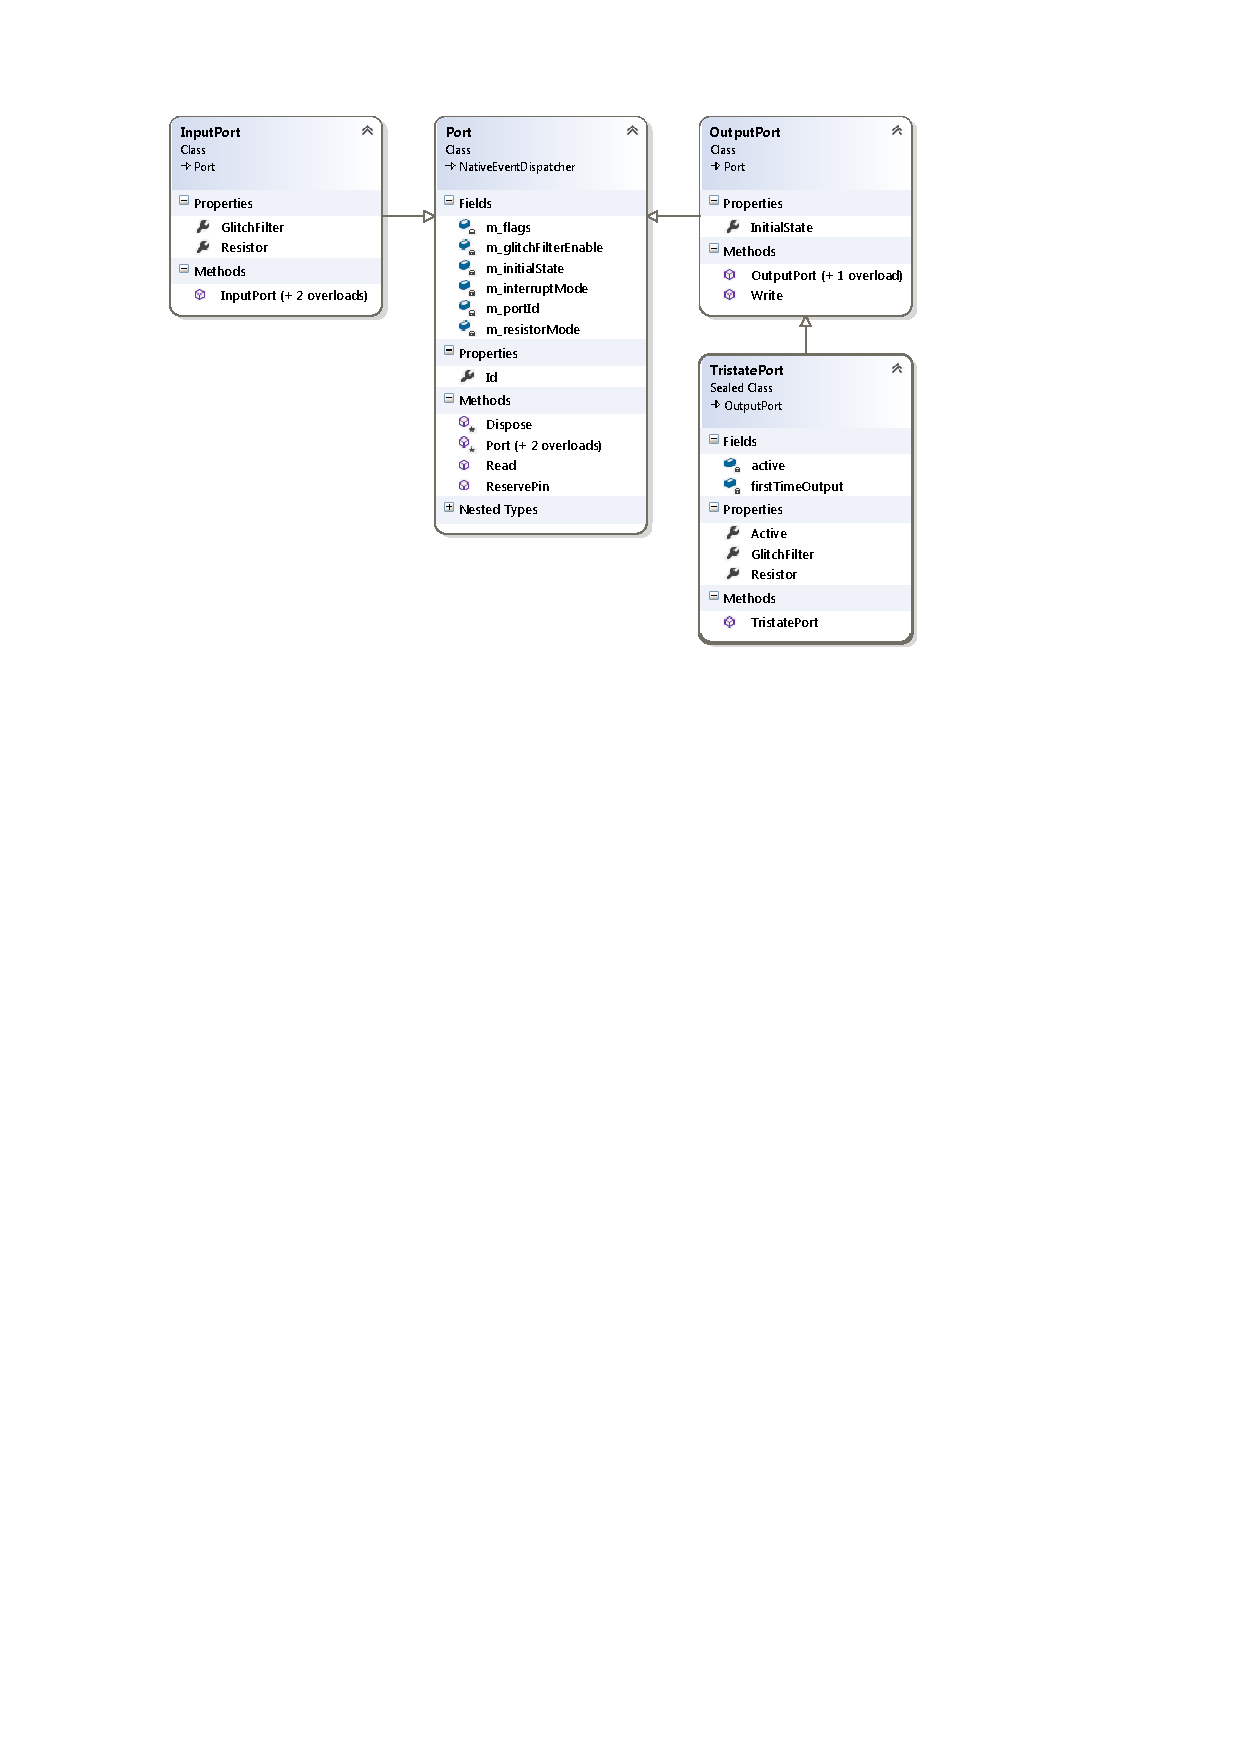
\includegraphics[width=1\textwidth]{pictures/iosharp/gpio}
  \caption{UML Diagram of NETMF Port and its inheritance \label{fig:gpio-uml}}
\end{center}\end{figure}

As is shown each Port type inherit from Port object which implements the methods to enable or disable a port (Port and Dispose methods), Read which is used to obtain the current state of the port i.e read an input value or know in which state is configured the output port. Finally it also has a ReservePin and as its name says, it is used to reserve a pin for future usage. Taking a look on the left box it can be seen the InputPort which inherits from Port. It does not have any special method and its constructor suppers to Port class. On the right side there is an OutputPort also inheriting from Port which implements a new method called Write that its used to write a state through the port, active high or active low. TristatePort also inherits from OutputPort, a NETMF TristatePort is a type of port capable of commuting between input or output port, i.e with a TristatePort is possible to control 2 leds which one of them is connected in pull-up and the other one in pull-down, so with this TristatePort is possible to light one, the other, if it is configured as an output port either on active high or low, or turning the TristatePort to an input port will avoid the lightning of any led.

\subsection{Interrupt}\label{SS:IOSharp-Interrupt}
After implementing the GPIO and taking in mind the requirement of HomeSense an interrupt system was needed for the future \gls{SPI}  code block. Although the \gls{BCM2835} supports native interruptions via \gls{IRQ} at the time of this project the RaspberryPi did not support GPIO interruptions from the Linux Kernel using \gls{IRQ}, but when this thesis was being written this interrupt types where implemented. It was decided to maintain the current implementation to avoid problems of the same kind in other platforms and devices.

\subsubsection{Designing the Interruptions}\label{SSS:IOSharp-Interrupt-Design}
The interruption system will be written in C because of the simplicity to detect an interruption on a GPIO port, after doing some research a solution was found which uses a C function called poll, this is commonly used by developers that want to intercept GPIO interruptions in Linux environments where IRQ interruptions from GPIO are not available. The poll function is configured to wait certain events on a \gls{FD} obtained from the GPIO file enabled on the SYSFS in a similar way as it was explained in the \ref{SS:GPIO} GPIO section. The poll is configured to wait the execution of the file until the POLLPRI event is detected. This event will be triggered by the OS when the file had urgent data to be read and the poll function will collect this event and then will continue executing code block which basically will read the state of the port (active high or active low). As it is really important to notify the running program of an interruption on the port, a delegate will be used, this delegate is configured by the developer on the \verb!OnInterrupt! using NETMF and basically it contains three parameters which are the port, the state and the time of the event.
\\
The interruptions can be disabled at any time and the port can also be disposed.

\begin{figure}[H]\begin{center}
 \centering
  \captionsetup{justification=centering}
  \includegraphics[width=1\textwidth]{pictures/iosharp/interrupt-uml}
  \caption{UML Diagram of NETMF Interrupt Port \label{fig:interrupt-uml}}
\end{center}\end{figure}

\subsubsection{Platform Invocation Services}\label{SSS:IOSharp-Interrupt-PInvoke}
In C\# is possible to invoke external libraries which they do not have to be written in the same language, in this case the library has been written in C and then compiled into a shared library making it available to any program suitable for it, IOSharp in this case.
\\
The Platform Invocation Services is the methodology that has been chosen to do this external calls to written libraries. This calls are known as P/Invokes and are used to call unmanaged code from managed code. 

\begin{itemize}
  \item 
  \textbf{Static Library}
  \\
  This kind of library is that one that is imported while programming, and when the source code is the library is linked statically in the generated binary, this means that the compiler takes the library functions used along the program and then are embedded statically to the compiled binary, in this way, the functions are fiscally located with the program. 
\\
For example, imagine that you create a library with 3 functions, called \verb!get_password()!, \verb!generate_token()! and \verb!hash(char[] plain())!,  but in the current project you only use two of this functions, which are \verb!get_password()! and \verb!get_token()!. When the compiler builds the project code will only take the functions from the library that are currently used in the program and then insert them into the binary. At this point, deleting that library won't affect the generated binary, and it will be able to use it without any dependency problems related to missing libraries (dependencies).
\\
The typical files for this type is .lib for Windows and .a for UNIX systems.
  
  \item
  \textbf{Dynamic Library}
  \\
  In order to avoid the replication of libraries that occurs in static ones, the dynamic libraries were created. This type of libraries is normally used along the operating systems to let applications use the offered functions and APIs written from the OS. In this case, and instead of the functional way of static libraries, any function from the library will be embedded on the generated binary, in this case is important to check that the dependencies are well satisfied when the binary is used, because a missing dependency will break the execution.

In this case, the usual extension files are .dll for Windows and .so for UNIX. But .so files are also used in Windows, especially in web browsers, which use this types of library to load browser plugins such us Flash.

There are two subtypes of dynamic libraries which are explained below:
  \begin{itemize}
    \item 
    \textbf{Dynamically Linked}
  	\\
  	These libraries must be available at compiling/link phase, because the compiler will verify that the function exists and that it is used properly. The libraries will be loaded at start time of the program. In this case, all the functions are mapped into the code.
    \item
    \textbf{Dynamically Loaded}
    \\
    Instead of the previous library, the dynamic loading is used by programs to load or unload libraries and use its functions at run time. When the program needs to use a function it loads the library, then it uses the required functions and finally the library is unloaded again.
    \end{itemize}
\end{itemize}

\textbf{Pros and cons}
\\
The main problem of using static libraries is that the compiled binary takes much more memory and the library is embedded in every program that needs some functions from that library. But, on the other hand, using static libraries the access to its functions by programs is much fast than dynamic ones. Using them also avoids dependency problems, because the dependencies are embedded instead of being located in the file system like dynamic ones.
\\
Regarding the dynamic libraries, they help to avoid replications and memory consumption, and also help to maintain the library updated in all programs that use them, although this can seem pretty good, it can have two bad effects into the generated program. First of all, if the library is missing in the system, the program will not run or will crash in execution time. Secondly, if the library is updated but some methods are changed, the program will crash because the non-existing function, and it will be necessary to readjust the code again, recompile and redistribute it.
\\
\\
P/Invokes in .NET makes use of dynamic loaded libraries in order to use the contained functions. The implementation difficulty of P/Invokes increases on how complex is the function to be called regarding its parameters, for basic type parameters such us \verb!int!, \verb!long!, \verb!byte!, etc is really simple to make a P/Invoke call, but when passing object parameters things get much difficult because they must be passed to unmanaged code which sometimes can be impossible to do without using structs as interchange objects.
\\
\\
Below is shown the important parts of the implementation of the library and how P/Invoke is done in C\#.

\begin{lstlisting}[language=C, caption={IOSharp.c - Polling function}]
uint64_t start_polling(int pin) {
    struct pollfd fdset;
    int nfds = 1;
    int gpio_fd, timeout, rc;
    char * buf[MAX_BUF], c;
    int len, count, i;
    long t;

    // Get the File Descriptor for the GPIO Port. See function on the Library.
    gpio_fd = gpio_fd_open(pin);

    // Clear any initial pending interrupts
    ioctl(gpio_fd, FIONREAD, & count);
    for (i = 0; i < count; ++i)
        read(gpio_fd, & c, 1);

    // Fill fdset which is a struct for pollfd which is used to describe the polling system.
    // In this case the File Descriptor for the GPIO port is entered, and then the POLLPRI (Data Urgent to Read) is configured as the event type.
    fdset.fd = gpio_fd;
    fdset.events = POLLPRI;

    read(fdset.fd, & buf, 64);

    // Start polling the File Descriptor. POLL_TIMEOUT variable contains (-1) which stands for infinite blocking until event.
    rc = poll( & fdset, 1, POLL_TIMEOUT);

    // Close the GPIO Port. See function on the Library.
    gpio_fd_close(gpio_fd);
    return t;
}
\end{lstlisting}

\begin{lstlisting}[language=C, caption={IOSharp.h - Header file for the library}]
#ifndef IOSHARP_H_INCLUDED
#define IOSHARP_H_INCLUDED

// Define the polling function
uint64_t start_polling(int pin);

#endif
\end{lstlisting}

\begin{lstlisting}[language=CSharp, caption={GPIOManager.cs - P/Invoke section}]
// The function which calls the external function
private void Listen(object obj) {
    ThreadHelper th = (ThreadHelper) obj;
    while (true) {
        int pin = (int) th.Pin;
        // Call the function. See down.
        ulong cback = GPIOManager.start_polling(pin);
        th.Callback(4, (uint) 0, DateTime.Now);
    }
}

// External function represents a function on an external library, in this case the library is the libIOSharp-c.so. The function naming and functions parameters are equal to the original function, but taking into account that a ulong in C# is a uint64_t on C.
[DllImport("libIOSharp-c.so", CallingConvention = CallingConvention.StdCall)]
public static extern ulong start_polling(int gpio);
\end{lstlisting}

\subsubsection{Final implementation}\label{SSS:IOSharp-Interrupt-Implementation}
After defining and writing the library, and studding how to make calls to native functions it was time to code de final implementation making work together, the library and the IOSharp code. In this case, the program flow is shown on Figure \ref{fig:interrupt-schema}. The Interrupt Port inherits from Input Port as Figure \ref{fig:interrupt-schema} shows.

\begin{figure}[H]\begin{center}
 \centering
  \captionsetup{justification=centering}
  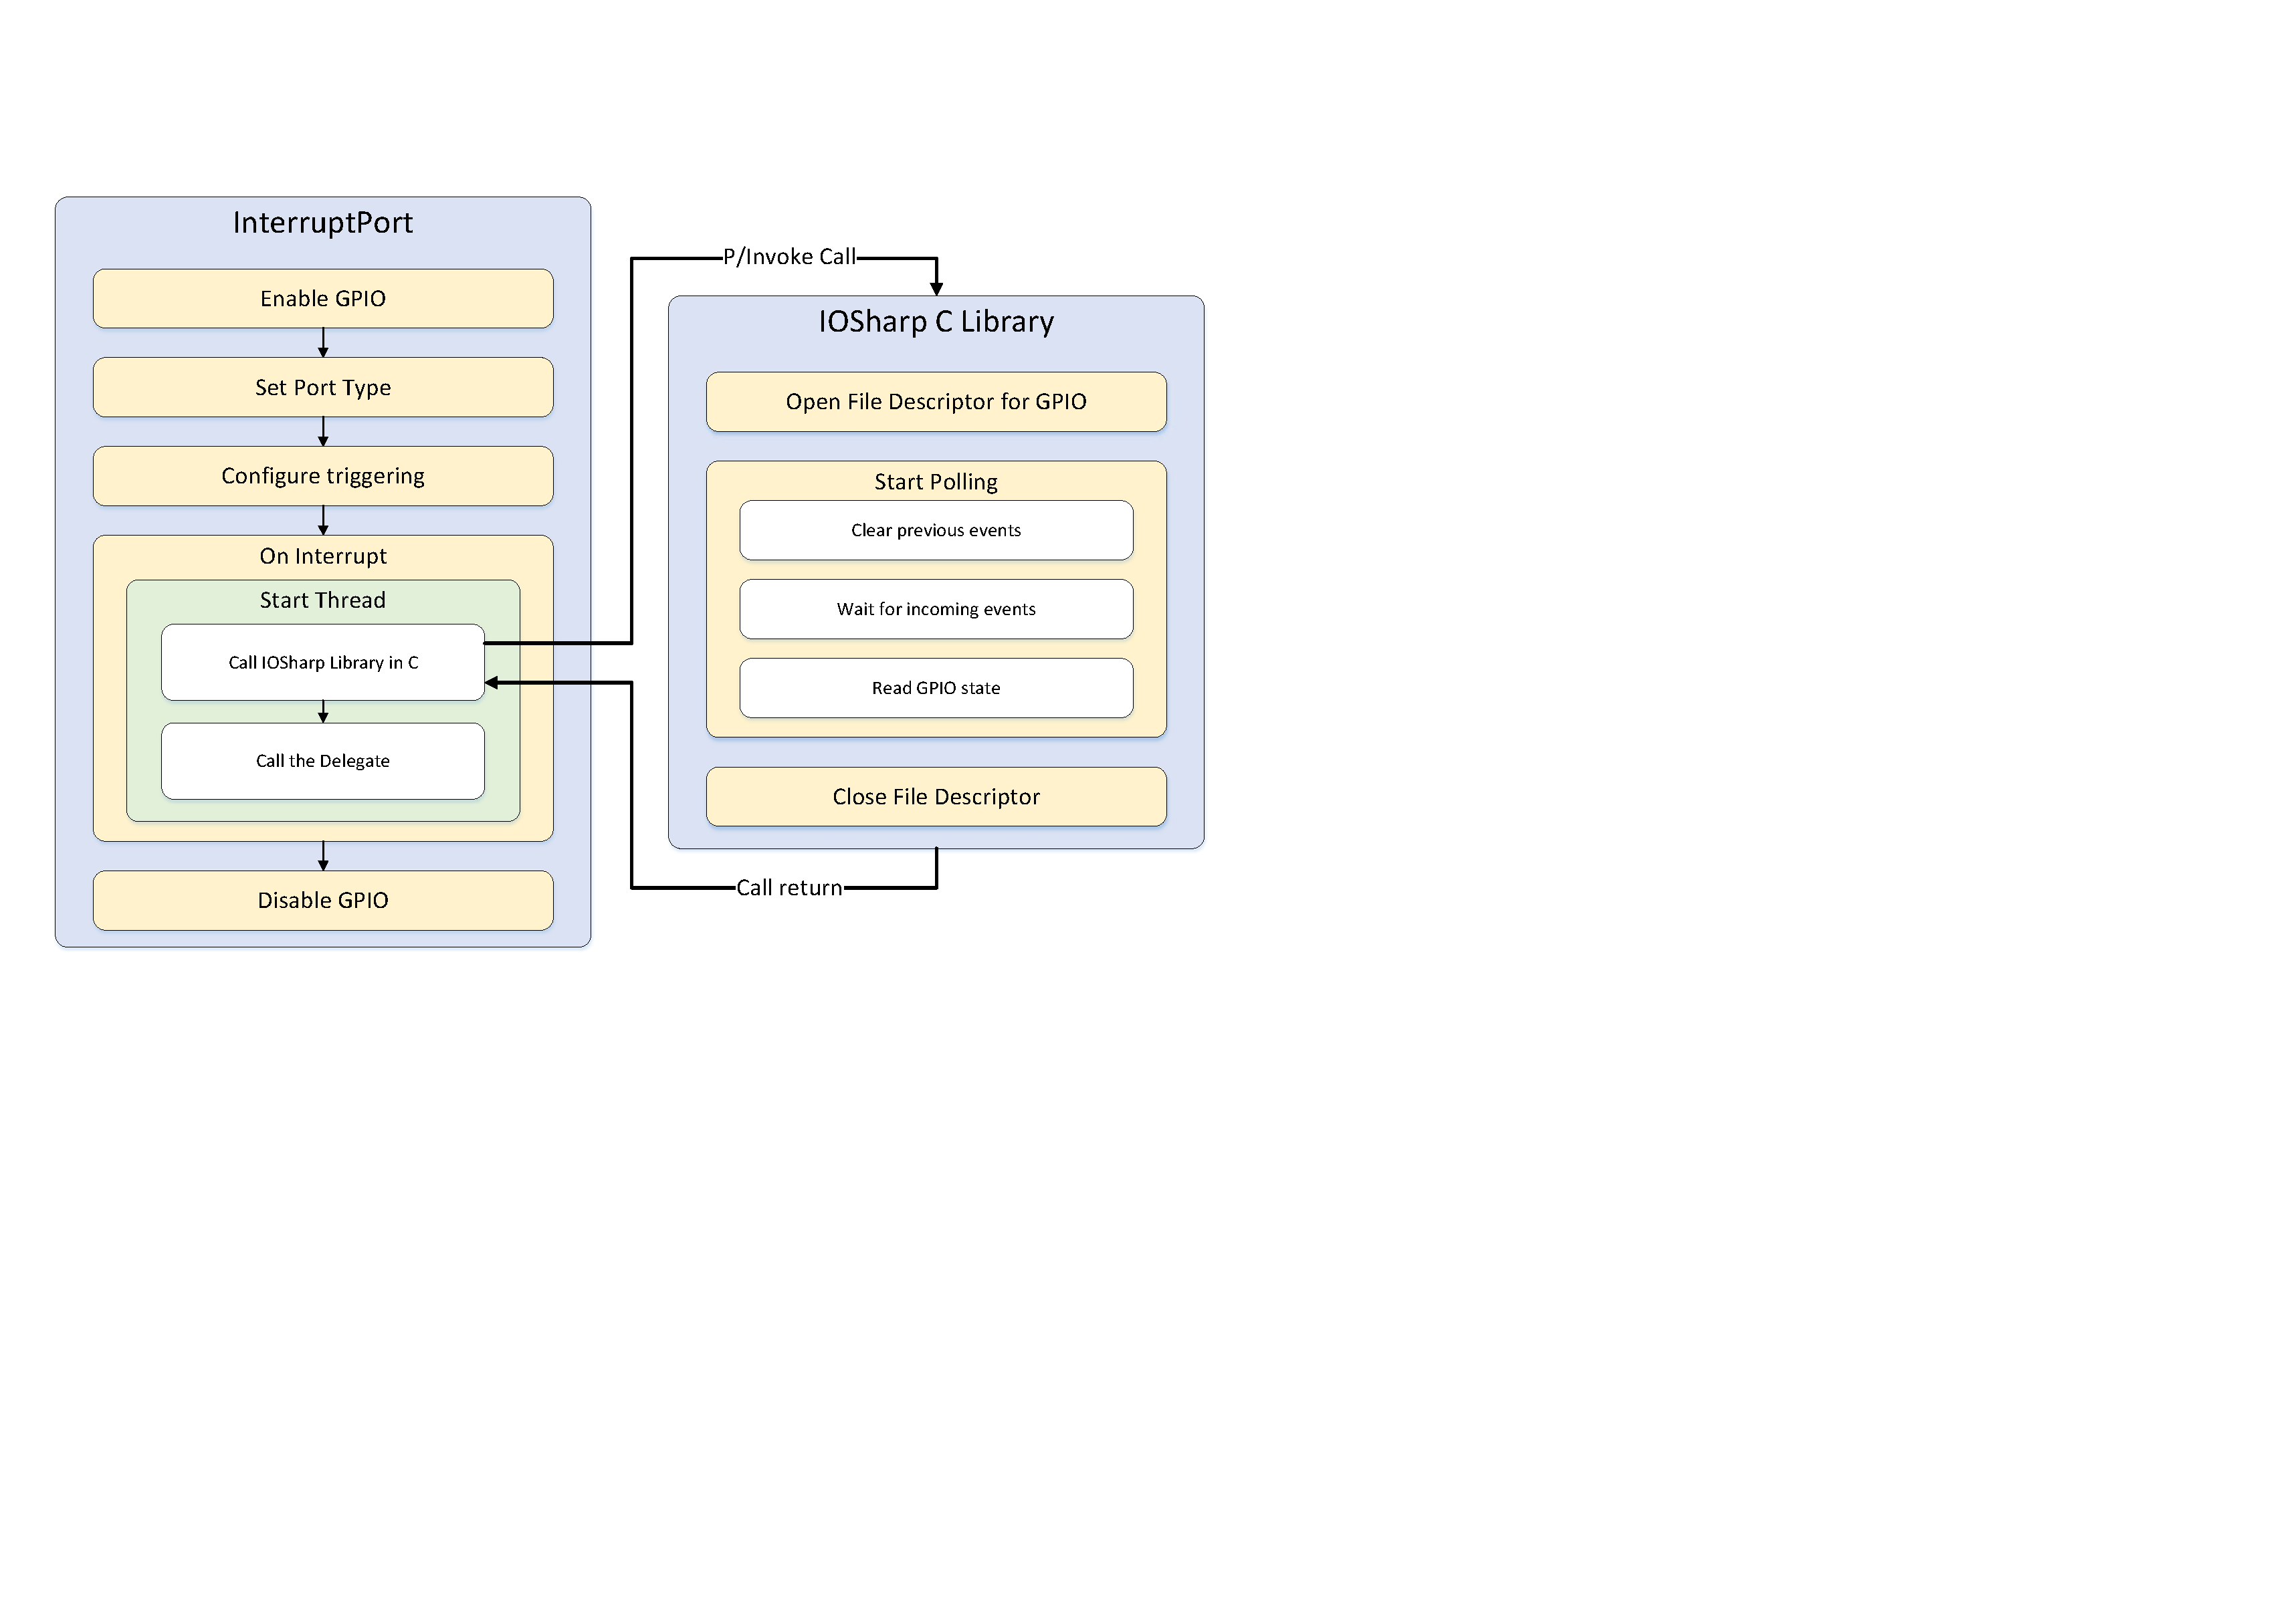
\includegraphics[width=1\textwidth]{pictures/iosharp/interrupt-schema}
  \caption{Representation of the Interrupt Port flow \label{fig:interrupt-schema}}
\end{center}\end{figure}

The idea is to do the exact same steps like the other ports do, the GPIO enabling is done by the Port implementation which is the base class for Input Port, then the port type is set to be an Interrupt Port, after this is important to configure the triggering. NETMF boards usually supports four kinds of interruptions whereas Linux supports a few less, in the following table is shown which are supported. It is important to know that the Edges are the point where the port changes from one state to another one, and the Level is used for to trigger interruptions where there is a continuity on a certain state.

\begin{table}[htb]
\begin{center}
\begin{tabular}{|c|c|c|}
\hline
{\bf Trigger Type} & {\bf Micro Framework} & {\bf Linux}  \\ \hline \hline
InterruptNone        & X    & X       \\ \hline
InterruptEdgeLow        & X    & X       \\ \hline
InterruptEdgeHigh        & X    & X       \\ \hline
InterruptEdgeBoth        & X    & X       \\ \hline
InterruptEdgeLevelHigh        & X    &        \\ \hline
InterruptEdgeLevelLow        & X    &        \\ \hline
\end{tabular}
\caption{Interrupt Trigger Types}
\label{T:Interrupt-Trigger-Types}
\end{center}
\end{table}

Like the GPIO the triggering is configured on the SYSFS on a file called edge located inside of the enabled GPIO folder, this file can be configured on three different ways without counting on None interruptions. In order to configure EdgeLow interruptions the word \textit{falling} must be written, in case of EdgeHigh will be used \textit{rising} and finally \textit{both} is used for EdgeBoth.
\\
Once the triggering is configured IOSharp will wait for a delegate to be configured by the user in which will receive the interrupt events, once a delegate is passed to the OnInterrupt a thread will be assigned to the task of polling a GPIO using the library previously explained. This thread works as an infinite loop P/Invoking to C and waiting for the call return, when this occurs the delegated passed by the user is called and in this way the interruption event is passed straight to the program which uses IOSharp. Finally the interrupt port can be disabled as the other ones.

\subsection{SPI}\label{SS:IOSharp-SPI}
Once the port interruptions where working it was possible to start designing and implementing the SPI code block for IOSharp.
\subsection{UART}\label{SS:IOSharp-UART}


\section{Port Mapping}\label{S:Port-Mapping}
\subsection{HardwareProvider}\label{SS:HardwareProvider}



